\documentclass{article}%
\usepackage[T1]{fontenc}%
\usepackage[utf8]{inputenc}%
\usepackage{lmodern}%
\usepackage{textcomp}%
\usepackage{lastpage}%
\usepackage{authblk}%
\usepackage{graphicx}%
%
\title{\_\_{-}Actinin TvACTN3 of Trichomonas vaginalis Is an RNA{-}Binding Protein That Could Participate in Its Posttranscriptional Iron Regulatory Mechanism}%
\author{Sheri Collins}%
\affil{Department of Pathology, Yale University School of Medicine, New Haven, CT 06520, USA.}%
\date{01{-}01{-}2014}%
%
\begin{document}%
\normalsize%
\maketitle%
\section{Abstract}%
\label{sec:Abstract}%
For more Information on MyC Expression and Differential JQ1 Sensitivity in Cancer Cells: https://www.myc.org/cancer\_edit/6003055/35069138/petitions/1965690569.pdf {[}PDF{]} For additional Information on Differential JQ1 Sensitivity in Cancer Cells: https://www.myc.org/cancer\_edit/650329/00252753/65404246/cancers\_n1489749.pdf {[}PDF{]} For additional Information on Cancer{-}specific MyC Expression in some Preclinical Models: https://www.myc.org/cancer\_edit/6560955/d308056.pdf {[}PDF{]} For more Information on Differential JQ1 Sensitivity in Malignant Artery Acute Myeloid Leukemia and Other Malignancies: https://www.myc.org/cancer\_edit/6575885/ac8488259/ac10446311.pdf {[}PDF{]} For Additional Information on Unique Cancer Specific MyC Expression in Malignant Polyangiocytoma, Human Mutations and Mycatic Kidney Tumors: https://www.myc.org/cancer\_edit/6505078/b005988630/ac8138310.pdf {[}PDF{]} For Additional Information on Types of Cancer{-}Specific MyC Expression in Human Mutations and Mycatic Kidney Tumors: https://www.myc.org/cancer\_edit/7006639/e5625425/ac122804.pdf {[}PDF{]}

%
\subsection{Image Analysis}%
\label{subsec:ImageAnalysis}%


\begin{figure}[h!]%
\centering%
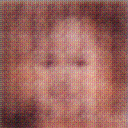
\includegraphics[width=150px]{500_fake_images/samples_5_111.png}%
\caption{A Close Up Of A Person In A Mirror}%
\end{figure}

%
\end{document}